\subsection{Flux}

O LIMS Flux foi utilizado para implementação dos recursos de workflows dinâmicos e da agregação de múltiplos BPMs para troca de informações entre eles. Sua utilização foi feita pela facilidade na criação de workflows dentro do próprio software e a alta personalização disponibilizada.

Como estes recursos alteram como a visualização de um BPM ocorre, foram necessário ajustes para que a implementação de tais recursos fosse feita de maneira correta e consistente, sem que a alteração na visualização deixasse o LIMS com vulnerabilidades de segurança e que as informações estivessem sempre disponíveis quando necessário.

\subsection{Alterações feitas para workflow dinâmicos}

Para que o Flux pudesse focar em uma atividade dentro do workflow, alteramos a definição de instância do programa. Anteriormente, instâncias eram definidas como o inicio do fluxo de trabalho do usuário para execução do BPM.

Com a implementação de workflows dinâmicos, foi necessário a utilização de instâncias como o ponto de partida de execução do usuário naquele momento, e não necessariamente o inicio do fluxo de trabalho. Instancias ainda podem ser utilizadas seguindo a definição anterior caso o usuário não selecione nenhuma atividade para ser focada (Ou selecione a atividade inicial original).

No software, instâncias ainda são criadas apenas para a atividade original, mas por baixo dos panos, para disponibilizar as informações para o usuário de maneira conveniente, é criado uma instância temporária onde a atividade inicial é a atividade selecionada pelo usuário, disponibilizando esta atividade centralizada como ponto de partida para sua execução.

É importante que estas instâncias auxiliares não sejam salvas para que não haja duplicação de dados do workflow e para não ocorrer alterações no BPM original. A ordem das atividades sempre deve seguir a estrutura original do BPM para manter o fluxo desejado quando ele foi modelado.

Se a estrutura do BPM mudar de uma maneira a disponibilizar atividades antes de uma dependência, isso pode causar um fluxo de trabalho errôneo que não segue as restrições modeladas quando o workflow foi implementado no sistema, e isso não pode ocorrer para que o BPM ainda esteja em conformidade com as diretrizes do laboratório.

Para selecionar qual atividade inicial será utilizada na visualização atual, foi alterada a interface para adicionar um seletor de atividades, disponibilizando todas as atividades que o usuário tem permissão de acessar em uma lista ordenada pelo nome da mesma. Nele, temos o nome de todas as atividades do workflow selecionado que o usuário tem a permissão de visualizar.

Caso o usuário não selecione nenhuma atividade, a atividade inicial utilizada será a padrão, deixando o workflow na visualização padrão (Como podemos ver na figura~\ref{fig:centrare_seletor_normal}). Quando o usuário seleciona uma atividade para ser focada, temos a alteração da interface para mostrar, como instância, todas as atividades executadas da atividade que o usuário selecionou no seletor (Como podemos ver na figura~\ref{fig:centrare_seletor_alterado}).

\begin{figure}
    \centering
    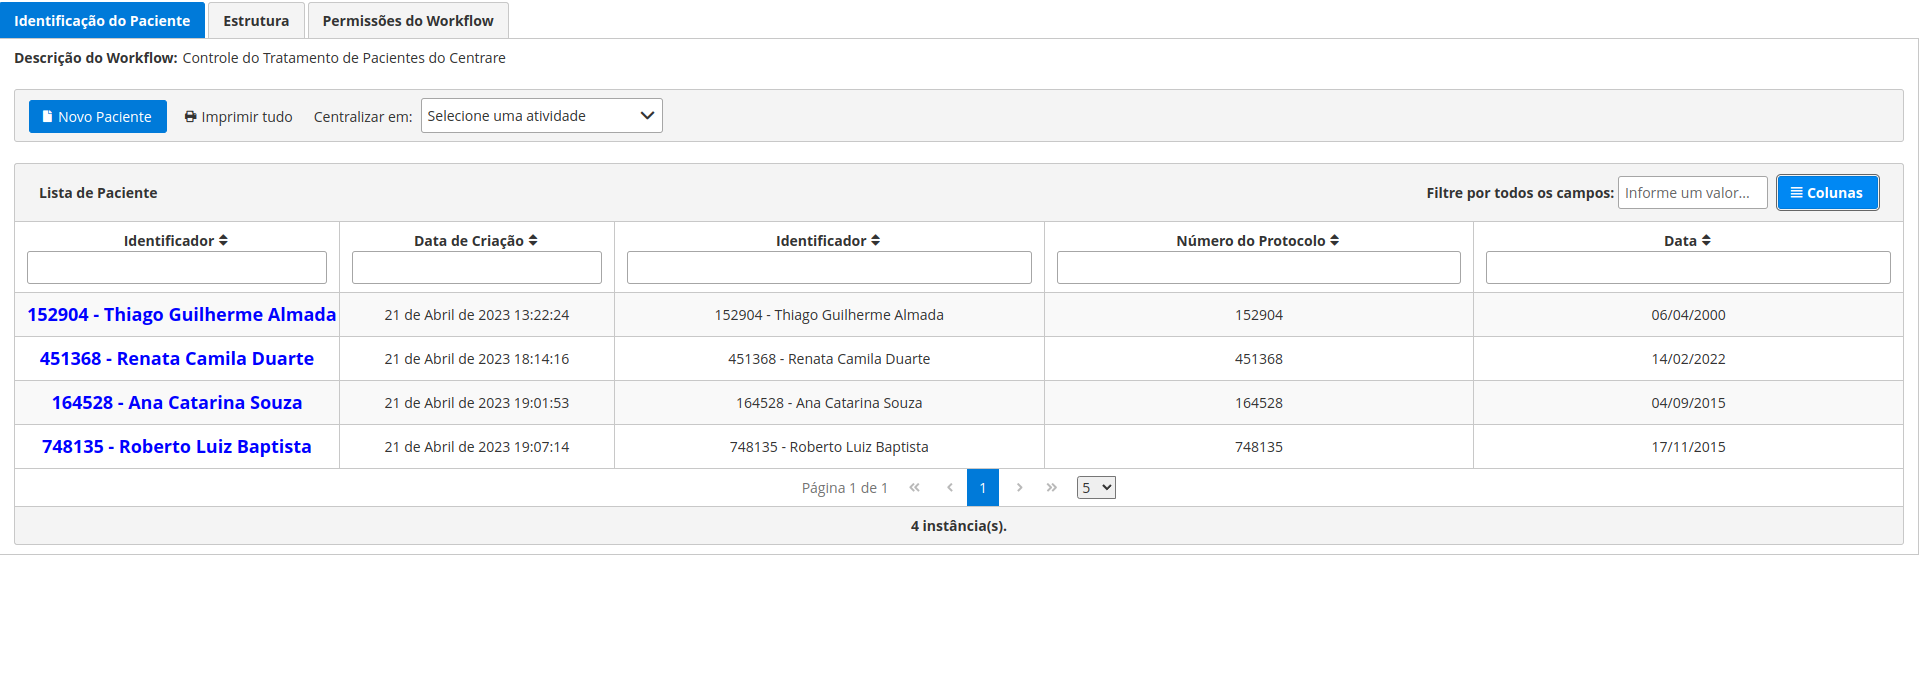
\includegraphics[width=1\textwidth]{imgs/CENTRARE/instanciaNormal.png}
    \caption{Nesta imagem podemos ver o workflow CENTRARE e o seletor de atividade inicial na parte superior da imagem. O seletor contém o escrito ``Selecione uma atividade", indicando que ele não foi alterado e a atividade que está sendo mostrada é atividade inicial original deste workflow.}
    \label{fig:centrare_seletor_normal}
\end{figure}

\begin{figure}
    \centering
    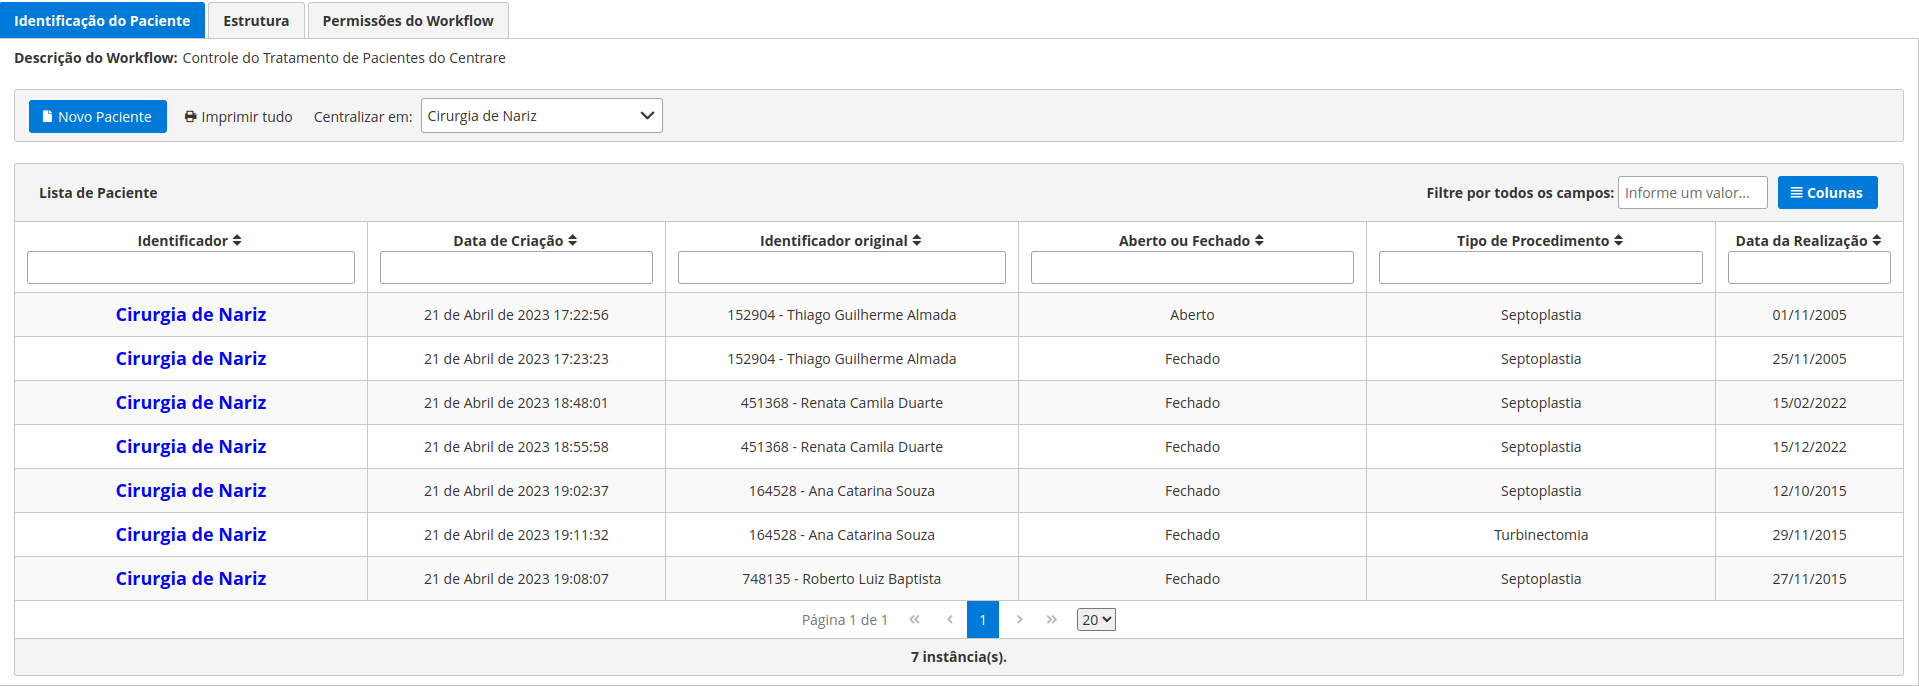
\includegraphics[width=1\textwidth]{imgs/CENTRARE/instanciaAlterada.png}
    \caption{Nesta imagem podemos ver o workflow CENTRARE e o seletor de atividade inicial na parte superior da imagem. O seletor contém o escrito ``Cirurgia de Nariz", indicando que o usuário selecionou a atividade com este nome para ser focada e utilizada como atividade inicial. Como podemos ver pela tabela, temos todas as atividades ``Cirurgia de nariz" representadas como instâncias do workflow.}
    \label{fig:centrare_seletor_alterado}
\end{figure}

A árvore de atividades também teve de ser alterada, com a criação de novos tipos de atividades: Atividades pai, ou atividades anteriores. Neste tipo de atividade (Identificados pela cor azul na figura~\ref{fig:centrare_tree_normal_altered}), não é possível executar novas atividades, sendo existentes apenas por motivos de disponibilização de informações pertinentes à execução atual.

Foi necessário a criação deste novo tipo de atividade para disponibilizar informações de atividades anteriores para o usuário, já que as informações podem ser pertinentes para o usuário.

Na mesma figura~\ref{fig:centrare_tree_normal_altered} temos as informações do paciente como primeira atividade da visualização original, podendo ser necessária para preenchimento de próximas atividades da atividade selecionada ``Cirurgia de Nariz".

\begin{figure}
    \centering
    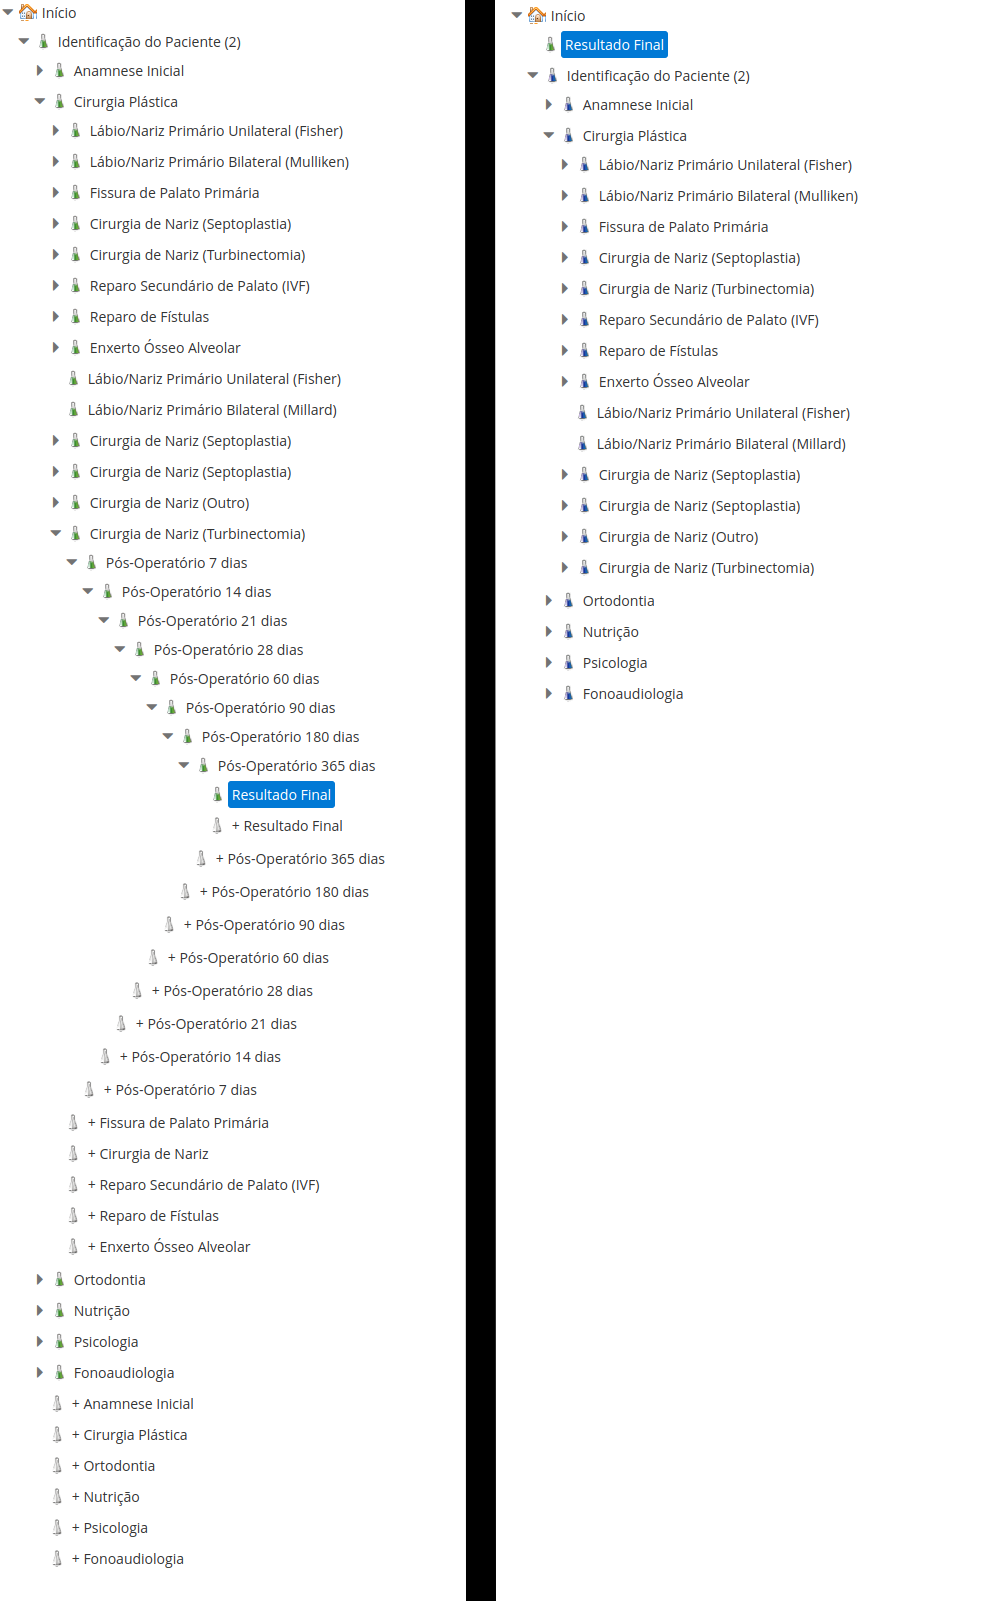
\includegraphics[height=1\textwidth]{imgs/CENTRARE/arvoreNormalEAlterada.png}
    \caption{Imagem demonstrando a árvore de atividades no software original (Esquerda) e a árvore de atividades alterada (Direita). Como podemos ver, a atividade selecionada na esquerda que está no meio do workflow é a mesma atividade selecionada na direita, que agora virou a atividade focada por seleção do usuário. Atividades pai são demonstradas em azul, disponibilizando todas as informações existentes mesmo com a alteração do foco do workflow.}
    \label{fig:centrare_tree_normal_altered}
\end{figure}

\subsubsection{Como funciona}

Quando o usuário seleciona a atividade desejada para ser a atividade inicial, a árvore de atividades é reajustada para que a atividade selecionada seja o foco principal da instância.

Para que isso ocorra, é necessário que a atividade selecionada se torne a atividade inicial, continuando com suas atividades filhas originais mas ganhando uma nova atividade filha: Sua atividade pai. As atividades que eram pais da atividade selecionada se tornam filhas da mesma para que essas informações estejam disponíveis para acesso e para manter a conformidade com a modelagem do BPM já existente.

Para isso, pode-se dizer que ocorre um ``giro" na árvore de atividades para a direita, tendo todas as atividades anteriores como atividades filhas da selecionada, mantendo a sub árvore de atividades originais intacta. Podemos ver esta característica na figure~\ref{fig:primeira_implementacao}.

\begin{figure}
    \centering
    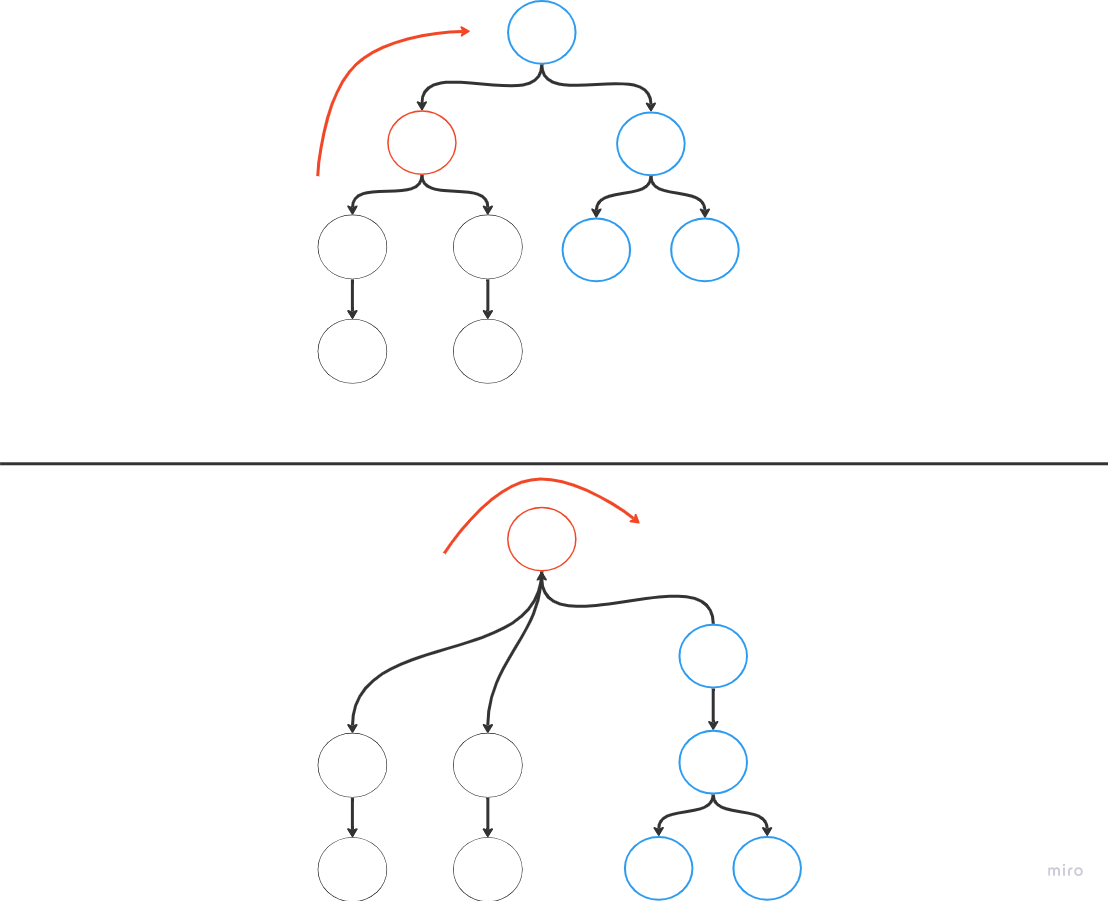
\includegraphics[width=1\textwidth]{imgs/Implementacoes/primeiraImplementacao.png}
    \caption{Representação da implementação de workflows dinâmicas. Na imagem de cima, podemos ver a implementação original de um workflow genérico que está prestes a ser reconstruído. A atividade em vermelho será utilizada como atividade focada apelo usuário. Com isso, a seta em vermelho representa o ``giro" que o workflow faz para que a atividade selecionada vire a primeira atividade do workflow.}
    \label{fig:primeira_implementacao}
\end{figure}

No Flux, esta funcionalidade faz com que atividades pai tenham uma cor diferente na interface do usuário (em azul na figura~\ref{fig:centrare_tree_normal_altered}) para que seja claro que as atividades vistas pelo usuário são atividades pai da atividade selecionada. Também é desabilitado a execução de novas atividades a partir das atividades pai.

\subsection{Alterações feitas para múltiplas atividades iniciais}

Segundo o BPMN, é possível que existam múltiplas atividades iniciais para um workflow, contanto que exista uma atividade inicial e uma atividade final para determinado tipo de execução de um BPM.

O Oracle BPM define que é necessário definir um ponto de início e um ponto de fim para um BPM, sendo possível a definição de múltiplos pontos iniciais, mas que cada ponto inicial criado defina uma instância diferente para execução o BPM~\ref{BPMNReference}.

\begin{figure}
    \centering
    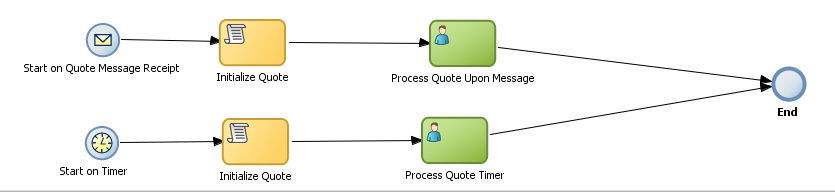
\includegraphics[width=1\textwidth]{imgs/BPM/Oracle_BPMN.png}
    \caption{Definição da Oracle sobre o funcionamento de múltiplas atividades iniciais em um processo~\cite{BPMNReference}. Um processo pode ser iniciado de diversas maneira, acarretando em um mesmo processo.}
    \label{fig:oracle_bpmn}
\end{figure}

Como um mesmo workflow pode ter troca de informações com alguma parte de outros workflows, foi idealizado uma nova funcionalidade para um workflow no Flux: Múltiplas atividades iniciais que compartilham atividades entre instâncias no meio de sua execução.

Com múltiplas atividades iniciais, é possível agregar diversos workflows que contém um fluxo de trabalho repetido (atividades que seguem o mesmo processo), com a disponibilização de atividades iniciais para usuários que têm permissão para executá-las.

Com a execução de dois workflows agregados, cada execução iniciando de uma atividade inicial diferente, é possível o compartilhamento das atividades que contém um processo idêntico entre os dois workflows agregados, disponibilizando as informações para as instâncias selecionadas.

Desta forma, aumenta-se a integração do sistema por haver a troca de informações entre processos de trabalho diferentes dentro de uma mesma organização, disponibilizando a cooperação entre usuários do mesmo sistema.

\subsubsection{Como funciona}

Para compartilhar atividades entre múltiplos workflows, é necessário que estes workflows estejam juntos em uma mesma modelagem com múltiplas atividades iniciais.

Para isso, foi alterado o editor de workflows já existente no Flux para que fosse possível criar múltiplas atividades iniciais, uma atividade inicial para cada workflow agregado.
Os workflows não precisam ter atividades compartilhadas para estarem juntos, eles funcionarão como workflows normais, com criação de instâncias e atividades da mesma maneira, apenas estando sob o mesmo nome de workflow e dentro da mesma interface que disponibiliza as informações de um workflow, disponibilizando recursos como busca de informações e geração de relatório dentro do mesmo workflow.

Quando for existir uma atividade compartilhada entre workflows, é necessário criar o fluxo de trabalho em um workflow, gerando todas as características necessárias para modelagem daquele processo. Logo após a criação das atividades, é necessário criar uma transição \textbf{(Explicar sobre transições anteriormente, junto a atividades e atributos)} de referência entre a atividade que será pai da atividade compartilhada em um workflow e a atividade compartilhada já criada no segundo workflow.

Existem dois tipos de compartilhamento: Um compartilhamento geral, onde a atividade será compartilhada entre todas as instâncias existentes assim que ela for criada e um compartilhamento seletivo, onde o usuário escolhe qual instância receberá as informações da atividade executada.

Nos dois casos, a disponibilização de atividades filhas da atividade compartilhada apenas não ocorre quando existir regras de permissões que não deixem certos usuários (ou grupos de usuários) acessar determinada atividade, caso contrário, todas as atividades e as informações contidas nelas serão compartilhadas.
Isso da uma ferramenta poderosa pela combinação do sistema de permissões e compartilhamento de atividades: A requisição de informações e a entrega das mesmas por dois setores diferentes de uma organização.

\subsubsection{Exemplos}

Vamos utilizar o exemplo de um pedido de exame em um workflow médico e o recebimento deste pedido de exame e execução do mesmo.
Um médico cria uma instância de paciente, cadastrando-o e seguindo o fluxo de trabalho comum de atendimento.
O laboratórios do hospital também tem seu próprio workflow, onde são cadastrados equipamentos para análise de amostras.
Antes, os workflows ficariam separados, sem comunicação entre eles.

Com o novo recurso implementado, os workflows podem compartilhar atividades como o pedido de exame: O médico tem a permissão de executar o pedido de exame, mas ele não aprova a atividade. Quem irá aprovar a atividade é o técnico de laboratório.

O técnico de laboratório recebe uma notificação que a atividade foi executada e pode aprovar ou reprovar a atividade.
Aprovando a atividade, o técnico continua com seu workflow normalmente até o resultado.
Caso o médico tenha permissão de visualizar as atividades entre o pedido de exame e resultado do exame, o médico poderá ver todo o processo de análise.
Caso contrário, o sistema de permissões controla o que o médico poderá ver, que será o pedido de exame e o resultado do exame.

Assim, a árvore de atividades, caso o médico tenha permissão de visualizar apenas o pedido de exame e a execução, fica da maneira representada na figura~\ref{fig:segunda_implementacao}

\begin{figure}
    \centering
    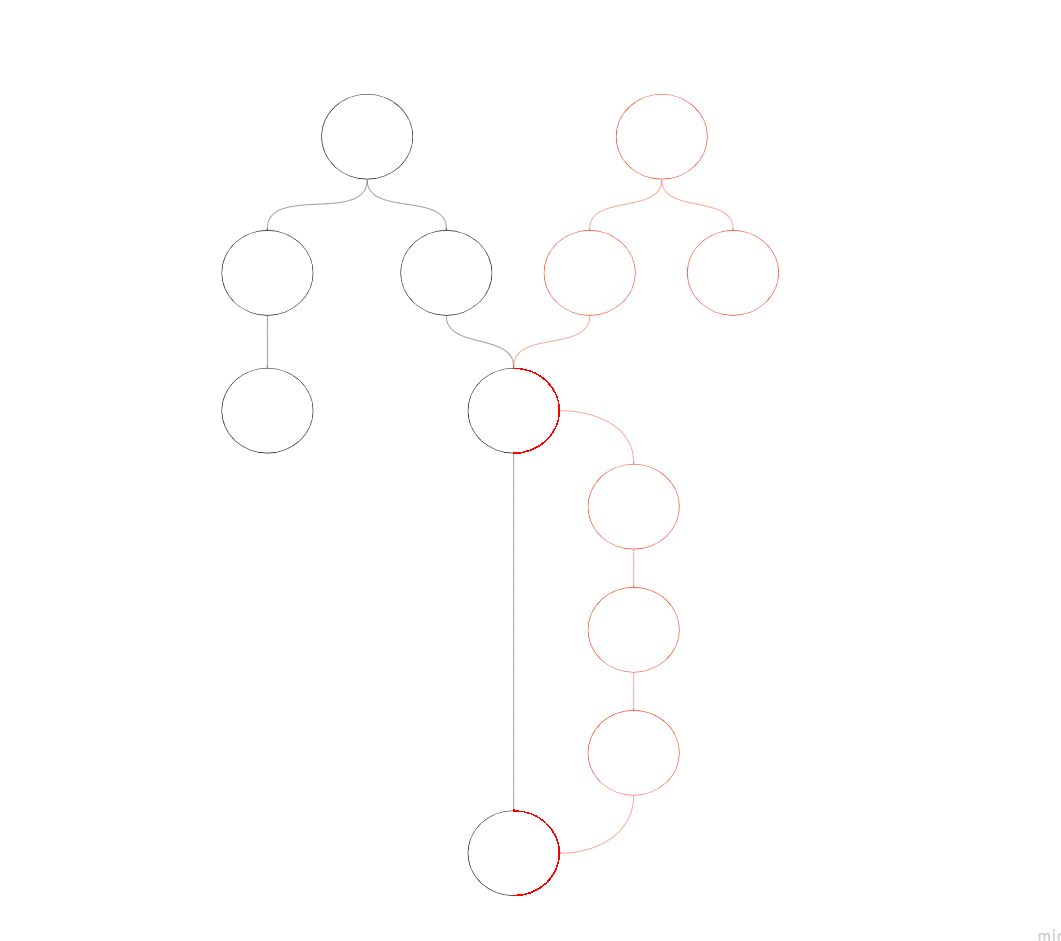
\includegraphics[width=0.5\textwidth]{imgs/Implementacoes/segundaImplementacao.png}
    \caption{Representação da implementação de múltiplas atividades iniciais. Neste exemplo, temos a instância de pacientes em preto e em vermelho temos o workflow do técnico de laboratório. Podemos ver que as atividades em preto e vermelho são compartilhadas, e apenas o técnico tem permissão de visualização das atividades entre o pedido de exame e o resultado do pedido.}
    \label{fig:segunda_implementacao}
\end{figure}

% Workflow grande feito no Flux